\documentclass[11pt,a4paper]{article}
\usepackage[margin=1in]{geometry}
\usepackage{amsmath,booktabs,graphicx,hyperref,natbib,algorithm,algpseudocode,float}
\usepackage[T1]{fontenc}
\usepackage{lmodern}
\graphicspath{{../figures/}}
\title{Supplementary Material:\\ Historical Path-Residual Guided Candidate Re-ranking for Catalog-Assisted S-Phase Repicking}
\author{}
\date{}
\begin{document}
\maketitle

\section{Algorithm 1: Historical path-residual candidate re-ranking}
\begin{algorithm}[H]
\caption{Historical path-residual candidate re-ranking (S phase)}
\begin{algorithmic}[1]
\Require waveform $w$ (current), catalog origin/location (event), station metadata, frozen train-only history store $H$, frozen PhaseNet STEAD weights, frozen DistanceMLP, $\lambda=(0.5,2.0,0.0)$, $K{=}5$, $k{=}50$
\State $p_S \gets$ PhaseNet\texttt{.annotate}($w$) remapped to waveform UTC grid
\State $C \gets$ top-$K$ peaks of $p_S$ (min distance 50, prominence 0.05, height 0.1; else global argmax)
\State $\tau^{\mathrm{base}} \gets$ DistanceMLP(distance, depth, \ldots)
\State $(n,r_{\mathrm{med}},r_{\mathrm{mad}}) \gets$ query $H$ with directed path key (train events only)
\If{$n < 5$ \textbf{or} residual-P MAD $> 1.0$}
  \State history\_available $\gets$ false; $\lambda_h \gets 0$
\Else
  \State $\tilde r \gets \mathrm{shrink}(r_{\mathrm{med}}, r_{\mathrm{global}}, n, k{=}50)$
  \State history\_available $\gets$ true
\EndIf
\State $\hat s,\sigma \gets$ convert $\tau^{\mathrm{base}}+\tilde r$ to sample index / $\sigma_{\mathrm{samp}}$
\For{candidate $j\in C$}
  \State $h_j \gets \exp(-\tfrac12((s_j-\hat s)/\sigma)^2)$
  \State $\mathrm{score}_j \gets \lambda_w\log(\pi_j+\varepsilon)+\lambda_h\log(h_j+\varepsilon)+\lambda_\rho\,\mathrm{norm}(\rho_j)$
\EndFor
\State \Return $\arg\max_j \mathrm{score}_j$
\end{algorithmic}
\end{algorithm}

\paragraph{Input provenance.}
Current waveform $\to$ PhaseNet probabilities and peaks;
event catalog $\to$ origin time/location for $\hat\tau$ and path key;
station metadata $\to$ path key / distance features;
frozen training history $\to$ residual median/MAD only (no val/test leakage).

\section{Stage 2 development results}
Stage~2 mixed fixed-eval (val+test) was used for $\lambda$ grids and shrinkage
search only. See project \texttt{artifacts/results/stage2/} and
\texttt{paper/tables/table\_subset\_stage2\_dev.csv}.
Do not treat Stage~2 as the paper primary test.

\section{Stage 4 auxiliary table}
Regenerate with \texttt{scripts/build\_paper\_assets.py}; CSV mirror:
\texttt{paper/tables/table\_stage4\_auxiliary.csv}.
Underpowered ($9$ events); bootstrap CIs include zero.

\section{Cross-weight transfer}
\texttt{paper/tables/table\_transfer\_weights.csv} (STEAD/ETHZ/SCEDC on Stage~4).

\section{Learned gate training details (ablation)}
Three seeds $\{42,123,2026\}$, fewer than $7$k parameters; mean gate $\approx 0.97$ on
Stage~3 test (near-PhaseNet collapse). C-class training examples rare.
Not recommended as main method.

\section{Oracle analysis}
Oracle nearest candidate in $K{=}5$: F1@$0.5{=}0.890$ on Stage~3.
Oracle PN/fixed selector: $0.720$.
Gap shows coverage vs selector headroom.

\section{Noise / fallback}
History-unavailable scoring sets $\lambda_h{=}0$ and matches PhaseNet probability
ranking among candidates (identity fallback).

\section{Frozen hyperparameters}
See \texttt{paper/tables/hyperparameters\_frozen.json}:
$K{=}5$, $k{=}50$, S $\lambda=(0.5,2.0,0.0)$, PhaseNet STEAD, pick threshold $0.3$,
min history $5$, MAD disable $1.0$\,s.

\section{Additional figures}
\begin{figure}[h]
\centering
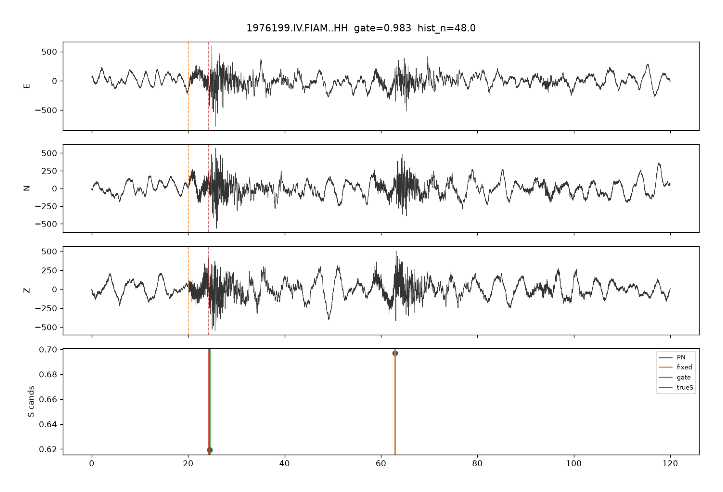
\includegraphics[width=0.85\linewidth]{fig_case_failure_fixed_wrong}
\caption{Negative-transfer / fixed-wrong case dump (Stage~3 frozen).}
\end{figure}
\begin{figure}[h]
\centering
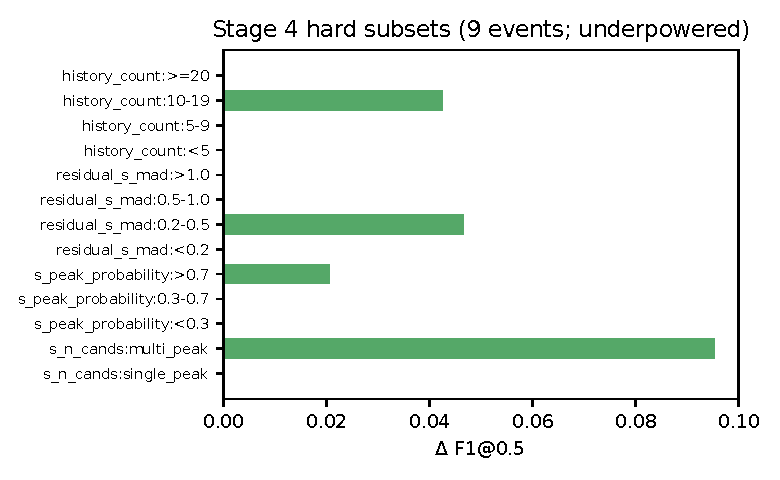
\includegraphics[width=0.7\linewidth]{fig_subset_gains_stage4_aux}
\caption{Stage~4 hard-subset deltas (underpowered).}
\end{figure}

\end{document}
